%%%%%%%%%%%%%%%%%%%%%%%%%%%%%%%%%%%%%%%%%%%%%%%%%%%%%%%%%%%%%%%%%%%%%%%%%%%%%%%
%% Where to Look Next — a data-landscape & opportunity scoping report for
%% strong-gravitational-lens discovery. Internal scoping report for the
%% agentic-lensing program (X. Huang group).
%%
%% Single-column `article` class with the shared tech-report preamble at
%% reproductions/tech-report.sty. Builds with vanilla TeX Live (>= 2022):
%%     make pdf      (pdflatex -> bibtex -> pdflatex x2)
%% Figures are produced by figures/make_figures.py (see Makefile `figures`).
%%%%%%%%%%%%%%%%%%%%%%%%%%%%%%%%%%%%%%%%%%%%%%%%%%%%%%%%%%%%%%%%%%%%%%%%%%%%%%%
\documentclass[11pt,letterpaper]{article}
\usepackage{../../reproductions/tech-report}
\usepackage{longtable}
\usepackage{array}
\usepackage{enumitem}
% Astronomy macros not in base LaTeX (tech-report only maps the Unicode glyphs).
\providecommand{\degree}{\ensuremath{^\circ}}
\providecommand{\arcsec}{\ensuremath{^{\prime\prime}}}

% RAG / availability / fit shorthands for the dense master table
\newcommand{\rgG}{\textcolor{green!55!black}{\textbf{G}}}
\newcommand{\rgY}{\textcolor{orange!85!black}{\textbf{Y}}}
\newcommand{\rgR}{\textcolor{red!72!black}{\textbf{R}}}
\newcommand{\survey}[1]{\textbf{#1}}

\title{Where to Look Next:\\
       A Data-Landscape \& Opportunity Scoping Report\\
       for Strong-Lens Discovery}
\author{Greg Benson \and (deep-research workflow)}
\date{6 June 2026}
\addbibresource{references.bib}

\begin{document}

\maketitle
\subtitle{Internal Scoping Report}

\begin{abstract}
The agentic-lensing program has searched the {DESI} Legacy optical-imaging footprints
(DR7--DR10, $\sim$19{,}000\,deg$^2$) and the {DESI} {DR1} spectroscopic catalogue (28\,M fibres)
about as hard as current methods allow, yielding $\sim$6{,}500 lens candidates across CNN
imaging finders, spectroscopic friends-of-friends search, and difference-imaging time-domain
search. This report asks the complementary question: \emph{which public telescope datasets have
\textbf{not} been exhaustively searched for strong lenses, or have no published lens results?}
We scanned the full multi-wavelength survey landscape with a deterministic multi-agent
research workflow (8 survey-family researchers, adversarial red-team verification of every
flagged opportunity, priority-scoring synthesis, completeness critic; 51 agents, $\sim$2.2\,M
tokens). Of 41 challenged opportunities, 34 were confirmed, 6 downgraded, and 1 refuted. The
headline finding is that the easy same-modality, in-footprint opportunities are gone --- the
major peer surveys (HSC PDR3, KiDS DR5, DES Y6, UNIONS, Euclid Q1) are already searched and
published --- and the genuine opportunities are: (i) \emph{virgin off-modality reservoirs}
(blind radio and submm/mm lens searches have \emph{never} been done at catalogue scale: VLASS,
the ALMA archive, ALMACAL, the faint-DSFG tail of Herschel/SPT-3G/ACT); (ii) \emph{drop-in
re-points} of the existing pipelines --- but \emph{all four} first-scan leads here (HST, VHS, GAMA,
DELVE~DR2) were downgraded or refuted on follow-up dives (\S\ref{sec:pressuretest},
\S\ref{sec:synth}), leaving only prototype-scale survivors (time-domain ATLAS/ZTF, DELVE~DR3-depth,
JWST COSMOS-Web, J-PLUS/S-PLUS); (iii) a
\emph{foundation-model re-mine} of the fibre-collision-blocked SDSS/BOSS spectroscopy; and
(iv) \emph{pre-positioning} for the megasurveys (Euclid DR1 Wide, Rubin/LSST, Roman,
DESI DR2). The lens-finding itself is out of scope; this report only maps where the un-mined
data is, how to access it, and how each opportunity fits the program's existing methods.
\end{abstract}

\paragraph{Provenance.} Every GREEN/YELLOW rating below was challenged by an independent
skeptic agent on four axes (\emph{already searched? public now? new sky? method fits?}); a GREEN
survives only with $\ge 2$ corroborating sources. Numbers are workflow estimates; the companion
Markdown report (\texttt{OPPORTUNITIES.md}) carries the same content with inline source links,
and the workflow script is archived at \texttt{workflow.js}.

% ===========================================================================
\section{Executive summary}
% ===========================================================================
The program's searched footprints are the \emph{baseline} (\S\ref{sec:baseline}), not
opportunities. The real opportunities fall into four buckets:
\begin{enumerate}[noitemsep]
  \item \textbf{Virgin off-modality reservoirs (highest novelty; needs new tooling).} Radio and
  submm/mm sky has never had a blind catalogue-scale strong-lens search --- only forecasts
  \citep{mckean2008,mccarty2024} and known-lens cross-matches \citep{martinez2024vlass} exist.
  \survey{VLASS} (33{,}885\,deg$^2$, public), the \survey{ALMA Science Archive}$+$\survey{ALMACAL}
  \citep{oteo2016almacal}, and the faint-DSFG tail of \survey{Herschel}/\survey{SPT-3G}/\survey{ACT}
  are genuine green fields. VLASS uniquely can also \emph{radio-confirm the program's existing
  $\sim$3{,}900 optical candidates}.
  \item \textbf{Drop-in re-points (public now).} \emph{This bucket did not survive scrutiny.} All
  four first-scan leads (\survey{HST archive}, \survey{VHS}, \survey{GAMA DR4}, \survey{DELVE DR2})
  were downgraded or refuted on dedicated deep-dives (\S\ref{sec:pressuretest}). The honest
  survivors are narrow and prototype-scale: time-domain diff-imaging on \survey{ATLAS}/\survey{ZTF}
  (the most robust), the \survey{DELVE DR3} depth gain $+$ low-$|b|$ frontier, \survey{JWST
  COSMOS-Web}, and \survey{J-PLUS}/\survey{S-PLUS}. There is no large fresh-public-data harvest with
  current methods (\S\ref{sec:synth}).
  \item \textbf{Foundation-model re-mine of legacy spectroscopy.} $\sim$5\,M public
  \survey{SDSS/BOSS/eBOSS} spectra cannot be pair-searched (the 55\arcsec/62\arcsec\
  fibre-collision radius forbids two fibres on a galaxy-scale pair) and the single-fibre
  emission-residual channel is exhausted \citep{bolton2006,brownstein2012,shu2017,talbot2021} ---
  but a SpectrumFM-style re-mine of the full spectral set is an open, build-once lever.
  \item \textbf{Pre-position for the megasurveys.} \survey{Euclid DR1 Wide} (public 2026-10-21),
  \survey{Rubin/LSST} (DP2 $\sim$2026\,Q3; world-public alerts), \survey{Roman HLWAS} (launch by
  2027; $\sim$160{,}000-lens forecast, \citealt{holloway2025roman}), and \survey{DESI DR2} spectra
  ($\sim$2027) are the eventual prizes.
\end{enumerate}

Figure~\ref{fig:priority} ranks the opportunities; Figure~\ref{fig:coverage} shows where the
virgin sky is. Table~\ref{tab:top} lists the highest-priority opportunities.

\begin{table}[t]
\centering\footnotesize
\caption{Top opportunities (priority score / tier / pipeline fit / access effort 1--5).}
\label{tab:top}
\begin{tabular}{@{}rllcl@{}}
\toprule
Score & Opportunity & Tier & Fit & One-line \\
\midrule
78 & VLASS (VLA Sky Survey) & new-tooling & New & 33{,}885\,deg$^2$ radio; no blind search ever; can radio-confirm optical lenses \\
78/75 & ALMA archive $+$ ALMACAL & new-tooling & New & Petabyte of mm/submm interferometry, never lens-searched \\
75/62$\to$\textbf{55/45}$^\ddagger$ & ATLAS/ZTF time-domain & drop-in & Diff & $^\ddagger$\emph{downgraded, strongest survivor} (\S\ref{sec:pressuretest}): reframe as a Rubin precursor (watchlist $+$ SpectrumFM gate) \\
$\sim$55$^\dagger$ & HST general archive (HLA) & drop-in & CNN & $^\dagger$\emph{downgraded on deep-dive} (\S\ref{sec:pressuretest}): completeness re-mine, tens--150 net-new \\
64$\to$\textbf{low}$^\ddagger$ & GAMA DR4 spectroscopy & \emph{refuted} & FoF & $^\ddagger$\emph{REFUTED} (\S\ref{sec:pressuretest}): two-fibre FoF can't reach $\theta_E\sim0.5$--$2\arcsec$; blended channel already done (Holwerda 2015) \\
63$\to$\textbf{low}$^\ddagger$ & VHS (VISTA Hemisphere) & \emph{refuted} & CNN(NIR) & $^\ddagger$\emph{REFUTED} (\S\ref{sec:pressuretest}): too shallow to see arcs (deflector-only) + not fresh; use DELVE~DR2 instead \\
66/63 & SPT-3G / Herschel faint tail & new-tooling & New & Large undelivered lensed-DSFG populations below the bright cut \\
62 / 61$\to$45$^\ddagger$ & JWST COSMOS-Web; DELVE DR2/3 & drop-in & CNN & JWST: deeper space. $^\ddagger$DELVE~DR2 \emph{downgraded} (\S\ref{sec:pressuretest}): $\sim$80--88\% already in Legacy DR10; DR3-depth $+$ low-$|b|$ are the levers \\
70--58 & Euclid DR1 / Rubin / Roman / DESI-DR2 & future-watch & --- & The megasurvey prizes; pre-position with early-access inquiries \\
\bottomrule
\end{tabular}
\end{table}

\begin{figure}[t]
\centering
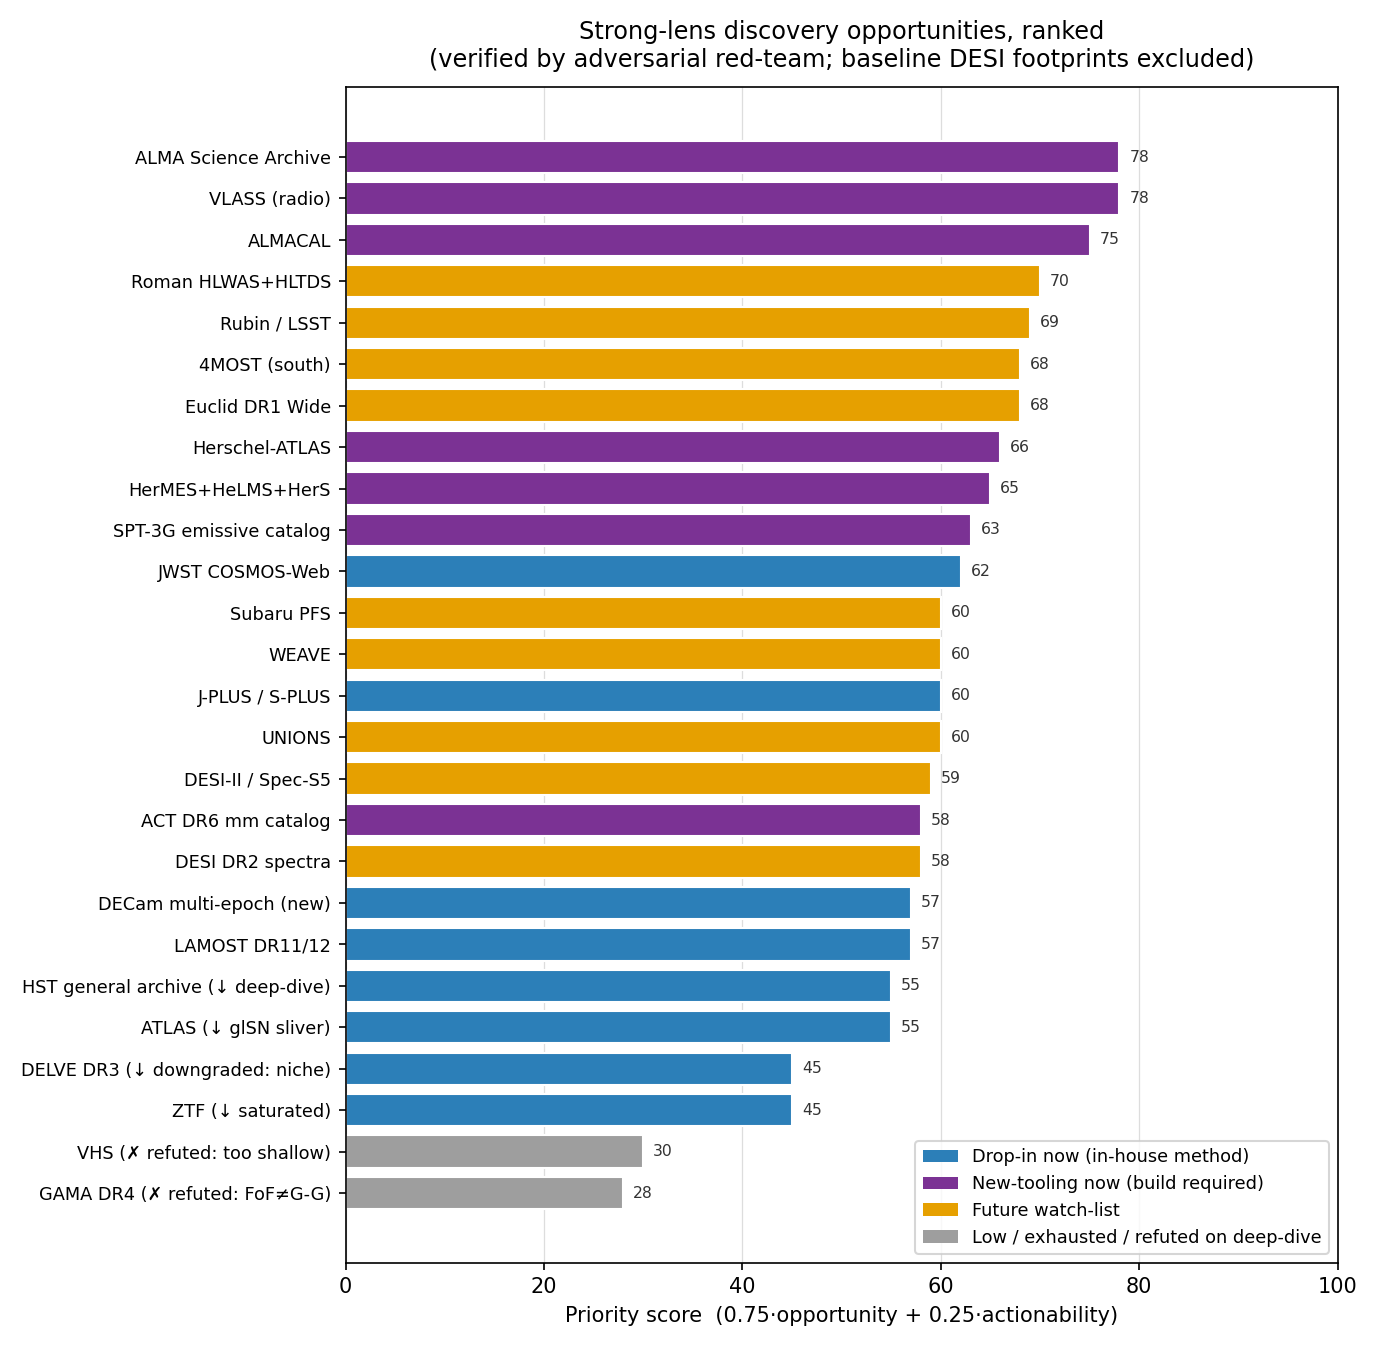
\includegraphics[width=0.92\linewidth]{figures/priority_ranking.png}
\caption{Verified opportunities ranked by priority score
($0.75\cdot\text{opportunity}+0.25\cdot\text{actionability}$), coloured by tier. Baseline DESI
footprints are excluded. Radio/submm reservoirs (purple) top the list on novelty despite
needing new tooling; the blue drop-ins re-use existing pipelines.}
\label{fig:priority}
\end{figure}

\subsection*{Pressure-test log (deeper follow-up dives)}\label{sec:pressuretest}
Individual opportunities are being stress-tested with dedicated 4-agent deep-dives (inventory $+$
prior-coverage $+$ pipeline $\to$ adversarial red-team); these \emph{supersede} the first-scan
ratings where they disagree. \textbf{HST general archive: DOWNGRADED} (first-scan score 68
$\to\sim$55). The dedicated dive (companion \texttt{HST\_ARCHIVE\_DEEPDIVE.md}, 6 corroborating
sources) found the ``hundreds, never ML-swept'' premise substantially false: HST is pencil-beam
($\sim$2.5--3\,deg$^2$ contiguous deep mosaic; whole-archive secure population only
$\sim$250--350), and the archive is \emph{not virgin} --- Hubble Asteroid Hunter~II
\citep{garvin2022} already crowd-scanned $\sim$27\,deg$^2$ (198 new) and COSMOS was already
CNN-searched \citep{pourrahmani2018} and JWST-mined (COWLS). Realistic \textbf{net-new secure
yield: tens--$\sim$150} via a completeness re-mine, not virgin discovery; best framing is a cheap
HST$\to$Euclid/Roman space-PSF CNN readiness prototype.

\textbf{VHS: REFUTED} (first-scan score 63; 8 corroborating sources; companion
\texttt{VHS\_DEEPDIVE.md}). Both load-bearing claims fail. \emph{(i) Depth kill-shot:} VHS
($J_{\rm AB}\sim20.8$, $K_{s,\rm AB}\sim20.0$; deepest $J\sim21.4$) is $\sim$3--4\,mag too shallow
and has no blue bands, so faint blue arcs fall below the limit --- a VHS CNN sees the deflector,
not the lens (no blind wide-NIR galaxy--galaxy catalogue has \emph{ever} been published; all
wide-NIR lensing is submm-counterpart or optical-colour use). \emph{(ii) Not fresh:} DECam reaches
$\delta=-90\degree$, and DELVE~DR2 ($\sim$21{,}000\,deg$^2$ griz) $+$ DES $+$ Legacy~DR10 already
blanket the southern sky 3--4\,mag deeper and mostly lens-searched, so net NIR-only fresh usable
sky is $\sim$0--10\% (the unusable plane). Realistic net-new yield $\sim$0--low-tens. The southern
residual it points to is re-running the optical CNN on \survey{DELVE DR2} griz, not a NIR search.
\textbf{GAMA DR4: REFUTED} (first-scan score 64; 6 sources; \texttt{GAMA\_DELVE\_DEEPDIVE.md}).
GAMA's multi-pass tiling does beat the fibre-collision wall, but that is a non-sequitur for
lensing: galaxy--galaxy lenses have $\theta_E\sim0.5$--$2\arcsec$, so the source lands inside one
$2\arcsec$ fibre --- the two-fibre FoF channel cannot reach them (only wide/group pairs). The
channel that works is the single-fibre blended spectrum, and \citet{holwerda2015} already did it
(104 candidates); the same channel on DESI just yielded 4{,}110 (arXiv:2512.04275). Net-new
galaxy--galaxy $\approx0$.

\textbf{DELVE DR2: DOWNGRADED} (first-scan score 61; 5 sources). The ``fresh sky'' premise fails:
DELVE DR2 tops out at $\delta\sim+30$ (below Legacy DR10's $+32$ ceiling), and Legacy DR10
\citep{inchausti2025} already CNN-searched $\sim$14{,}000\,deg$^2$ south of $+32$ \emph{and ingested
the same DELVE/DeROSITAS exposures}, so $\sim$80--88\% is the same photons already searched.
Genuinely fresh-and-deep residual is only $\sim$2{,}000--4{,}000\,deg$^2$ of low-$|b|$ sky; the real
levers are the \survey{DELVE DR3} deeper coadd ($\sim$0.5--0.7\,mag) and the low-$|b|$ frontier
(tens--few-hundred low-grade, eclipsed by Rubin within $\sim$2--3\,yr).

\textbf{ATLAS/ZTF time-domain: DOWNGRADED --- the strongest survivor} (first-scan score 75/62; 16
sources; \texttt{ATLAS\_ZTF\_DEEPDIVE.md}). The thesis fails on three of four axes but keeps a real
niche and a forward-looking role. ZTF's glSN alert content is \emph{saturated} --- a full-archive
search (Magee 2023) returned 0, an AMPEL pipeline runs live, the group's \emph{own} Park/Huang 2026
finder is validated on ZTF, and 4 brokers classify every alert; both real ZTF glSNe were caught live
by the magnification method, not at lens positions, so position-targeted diff-imaging adds $\ll1$.
Lensed-QSO discovery is blocked by the $<2\arcsec$ resolution wall (\,$\sim$90--95\% unresolved at
ZTF's $\sim2\arcsec$ PSF\,); net-new $\approx0$. ``Diff-imaging drops straight in'' is \emph{refuted}
--- ZTF/ATLAS already emit difference-image alerts $+$ forced photometry. ATLAS is the one genuine
under-searched glSN channel but is depth-capped to a handful of extreme events. \emph{What survives,
and uniquely, is a constructive reframing: a known-lens watchlist $+$ a SpectrumFM spectral gate
that doubles as a Rubin-era dress-rehearsal} (\S\ref{sec:synth}).

\textbf{Meta-finding (read first):} \emph{all five} current-data ``fresh public data, existing
method'' leads led with in the first scan (HST, VHS, GAMA, DELVE~DR2, ATLAS/ZTF) have now been
downgraded or refuted (2 refuted, 3 downgraded). The southern DECam optical sky, the DESI/SDSS
spectroscopy, \emph{and} the ZTF time-domain stream are far more thoroughly mined --- by the group
itself (Legacy DR10, Hsu~2025, Park/Huang~2026) and the community (HAH-II, Holwerda~2015, DESI
single-fibre, KiDS/HSC CNNs, Magee~2023, the Goobar group, 4 brokers) --- than a first-pass scan
credits, and each alternative modality hits a hard wall. \textbf{There is no large fresh-public-data
harvest reachable with current techniques}; the one lead that points somewhere constructive is the
ATLAS/ZTF$\to$Rubin precursor. See the synthesis in \S\ref{sec:synth}.

% ===========================================================================
\section{Scope \& baseline (what is excluded)}\label{sec:baseline}
% ===========================================================================
This report \emph{excludes} the footprints the program has already mined (indexed in
\texttt{reproductions/REPRODUCTIONS.md}); these are the baseline, not opportunities:
\begin{itemize}[noitemsep]
  \item \textbf{DESI Legacy Imaging DR7/8/9/10} (DECaLS$+$BASS$+$MzLS, grz/$+i$): optical-CNN
  finders \citep{huang2020,huang2021,storfer2024,inchausti2025} $\to$ $\sim$3{,}900 candidates.
  \item \textbf{DESI DR1 spectroscopy} (28\,M redshifts): spectroscopic FoF/pair \citep{hsu2025}
  $+$ quasar autocorrelation \citep{dawes2023} $\to$ $\sim$2{,}600 candidates.
  \item \textbf{DECam multi-epoch} over the lens footprint: difference imaging
  \citep{sheu2023,sheu2024a}.
  \item \textbf{HST/MAST, Keck NIRES, VLT/MUSE, Euclid Q1}: follow-up/confirmation only.
\end{itemize}
The three in-house methods (used for the \emph{fit} column): \textbf{optical-cnn} (CNN on
$grz(i)$ cutouts; retrains for NIR/space PSF as a config change), \textbf{spectro-fof}
(redshift-pair/emission-residual search), \textbf{diff-imaging} (multi-epoch). Anything else
(radio source-matching, uv-plane lens modelling, submm DSFG selection, IFU, astrometric
multiplets, foundation-model re-mine) is \textbf{new-tooling}.

\paragraph{Rating rubric.} \textbf{RAG (verified):} \rgG~largely unsearched \& public;
\rgY~partial / searched-but-unpublished / future-but-high-value; \rgR~exhausted or unviable.
\textbf{Priority} $=0.75\cdot$opportunity$+0.25\cdot$actionability (opportunity weighs verified
RAG, fresh sky, yield; actionability weighs pipeline fit, access effort, public availability ---
so scientific opportunity dominates convenience). \textbf{Tier:} drop-in-now / new-tooling-now /
future-watch / low.

% ===========================================================================
\section{Master opportunity table}
% ===========================================================================
All 55 datasets, ranked by priority (Table~\ref{tab:master}). Avail: P=public, E=embargoed,
F=future. Fit: CNN=optical-cnn, FoF=spectro-fof, Diff=diff-imaging, New=new-tooling.

{\footnotesize
\begin{longtable}{@{}r c c c >{\raggedright\arraybackslash}p{3.3cm} >{\raggedright\arraybackslash}p{6.2cm}@{}}
\caption{Master opportunity table (verified, priority-ranked).}\label{tab:master}\\
\toprule
Pri & RAG & Fit & Av & Dataset & Note \\ \midrule
\endfirsthead
\multicolumn{6}{c}{\tablename~\thetable{} -- continued}\\ \toprule
Pri & RAG & Fit & Av & Dataset & Note \\ \midrule
\endhead
\bottomrule
\endfoot
78 & \rgG & New & P & VLASS & 33{,}885\,deg$^2$ radio; no blind lens search ever \\
78 & \rgG & New & P & ALMA Science Archive & PB interferometry, never systematically lens-searched \\
75 & \rgG & New & P & ALMACAL & $\sim$1{,}000 calibrator sightlines, virgin (no proprietary period) \\
75$\to$55$^\ddagger$ & \rgY & Diff & P & ATLAS (Tonry) $\ddagger$ & $^\ddagger$\emph{downgraded} (\S\ref{sec:pressuretest}): the one genuine glSN gap, but depth-capped to a handful of extreme-mag events \\
70 & \rgY & CNN & F & Roman HLWAS$+$HLTDS & $\sim$160{,}000-lens forecast (launch by 2027) \\
69 & \rgY & Diff & E & Rubin / LSST & $\sim$10$^5$ full survey; world-public alert stream \\
68 & \rgY & CNN & F & Euclid DR1 Wide & $\sim$7{,}000 A/B forecast; public 2026-10-21 \\
$\sim$55$^\dagger$ & \rgY & CNN & P & HST general archive (HLA) & $^\dagger$\emph{downgraded} (\S\ref{sec:pressuretest}): not virgin (HAH-II scanned $\sim$27\,deg$^2$); tens--150 net-new via re-mine \\
68 & \rgY & FoF & F & 4MOST (south) & only large fresh \emph{southern} spectroscopy \\
66 & \rgY & New & P & Herschel-ATLAS & faint sub-threshold DSFG residual O(10$^3$) \\
65 & \rgY & New & P & HerMES$+$HeLMS$+$HerS & faint-DSFG residual \\
64$\to$low$^\ddagger$ & \rgR & FoF & P & GAMA DR4 $\ddagger$ & $^\ddagger$\emph{REFUTED} (\S\ref{sec:pressuretest}): FoF can't reach G-G $\theta_E$; blended already done (Holwerda 2015); $\sim$0 net-new G-G \\
63$\to$low$^\ddagger$ & \rgR & CNN & P & VHS $\ddagger$ & $^\ddagger$\emph{REFUTED} (\S\ref{sec:pressuretest}): $\sim$3--4\,mag too shallow for arcs (deflector-only); DECam covers the sky deeper \\
63 & \rgY & New & P & SPT-3G emissive catalog & deeper mm; 4{,}303 candidates already extracted \\
62 & \rgY & CNN & P & JWST COSMOS-Web & re-searchable deeper than the COWLS visual pass \\
62$\to$45$^\ddagger$ & \rgY & Diff & P & ZTF $\ddagger$ & $^\ddagger$\emph{downgraded} (\S\ref{sec:pressuretest}): glSN field saturated (Magee$\to$0; Park/Huang 2026; 4 brokers); lensed-QSO blocked by $<2\arcsec$ wall; net-new $\approx0$ \\
61$\to$45$^\ddagger$ & \rgY & CNN & P & DELVE DR2/DR3 $\ddagger$ & $^\ddagger$\emph{DOWNGRADED} (\S\ref{sec:pressuretest}): $\sim$80--88\% already in Legacy DR10; DR3-depth $+$ low-$|b|$ frontier are the real levers \\
60 & \rgY & CNN & E & UNIONS & z-band/footprint/CFIS-u residual (GLUE I ran deep gri) \\
60 & \rgY & CNN & P & J-PLUS / S-PLUS & novel 12-band narrow-band selection \\
60 & \rgY & FoF & E & WEAVE & fresh northern spectroscopy (annual DRs) \\
60 & \rgY & FoF & E & Subaru PFS & $\sim$100\% fresh as spectroscopy \\
59 & \rgY & FoF & F & DESI-II / Spec-S5 & deeper/higher-$z$ over DESI footprint (future) \\
58 & \rgY & FoF & E & DESI DR2 spectra & $\sim$50\% new objects; $\sim$2027 \\
58 & \rgY & New & P & ACT DR6 mm catalog & faint lensed-DSFG residual over 19{,}000\,deg$^2$ \\
57 & \rgY & FoF & P & LAMOST DR11/12 & $\sim$30\% fresh objects vs SDSS NGC \\
57 & \rgY & Diff & P & DECam multi-epoch (new) & DES-SN $+$ DELVE-DEEP $+$ archive; fresh epochs \\
56 & \rgY & CNN & P & VISTA VIKING & NIR modality gap ($=$KiDS sky) \\
56 & \rgY & New & P & ASKAP EMU $+$ RACS & $\sim$20{,}000\,deg$^2$ fresh southern radio \\
54 & \rgY & CNN & F & HSC-SSP PDR4 & increment over PDR3 (release date unknown) \\
53 & \rgY & CNN & P & UKIDSS LAS & modest NIR residual \\
53 & \rgY & New & P & Planck PHz/PCCS2 & all-sky submm residual \\
52 & \rgY & CNN & P & VIDEO & deep NIR, tiny area \\
51 & \rgY & CNN & P & VST-ATLAS DR4 & u-band differentiator; $\sim$0\% fresh sky \\
50 & \rgY & New & P & LOFAR LoTSS DR2 & sub-arcsec ILT uv-plane = high ceiling (unbuilt) \\
50 & \rgY & New & P & ALMA Lensing Cluster Survey & cluster-field mm; low galaxy-scale content \\
48 & \rgY & New & P & SDSS/BOSS/eBOSS ($+$MaNGA) & foundation-model re-mine only (fibre-collision-blocked) \\
48 & \rgY & New & P & MeerKAT MIGHTEE/MALS & small/medium-area radio \\
47 & \rgY & New & P & Gaia GraL/GravLens & astrometric lensed-QSO; largely worked \\
46 & \rgR & CNN & P & SkyMapper DR4 & \emph{refuted}: $\sim$1.5\arcsec\ seeing / shallow $\Rightarrow$ unviable \\
44 & \rgR & CNN & P & KiDS DR5 & searched; incremental only \\
44 & \rgY & New & P & Gaia Photometric Alerts & bright limit dominates \\
42 & \rgR & CNN & P & JWST other deep fields & now swept (AnomalyMatch / COWLS / Nagam 2025) \\
41 & \rgR & CNN & P & Pan-STARRS1 3$\pi$ DR2 & shallow, heavily overlapped \\
36 & \rgR & CNN & P & HSC-SSP PDR3 & searched end-to-end (SuGOHI/HOLISMOKES) \\
35 & \rgR & CNN & P & DECaLS-south DR10 $i$-band & program baseline \\
35 & \rgR & FoF & P & 2dFGRS $+$ 6dFGS & shallow/low-$z$ \\
34 & \rgR & CNN & P & HST COSMOS (ACS) & searched \\
34 & \rgR & FoF & P & DEVILS DR1 & tiny area \\
33 & \rgR & CNN & P & Euclid Q1 & exhausted benchmark \\
32 & \rgR & CNN & P & DES Y6 / DR2 & exhausted (Space Warps / Jacobs / Rojas) \\
32 & \rgR & CNN & P & Southern Pan-STARRS strip & $\sim$0\% fresh \\
32 & \rgR & CNN & P & UltraVISTA & over-studied COSMOS \\
30 & \rgR & New & P & SPT-SZ DSFG sample & bright selection exhausted \\
29 & \rgR & New & P & FIRST $+$ NVSS (CLASS/JVAS) & legacy; low residual \\
23 & \rgR & New & P & VVV / VVVX & Zone of Avoidance \\
\end{longtable}}

\begin{figure}[t]
\centering
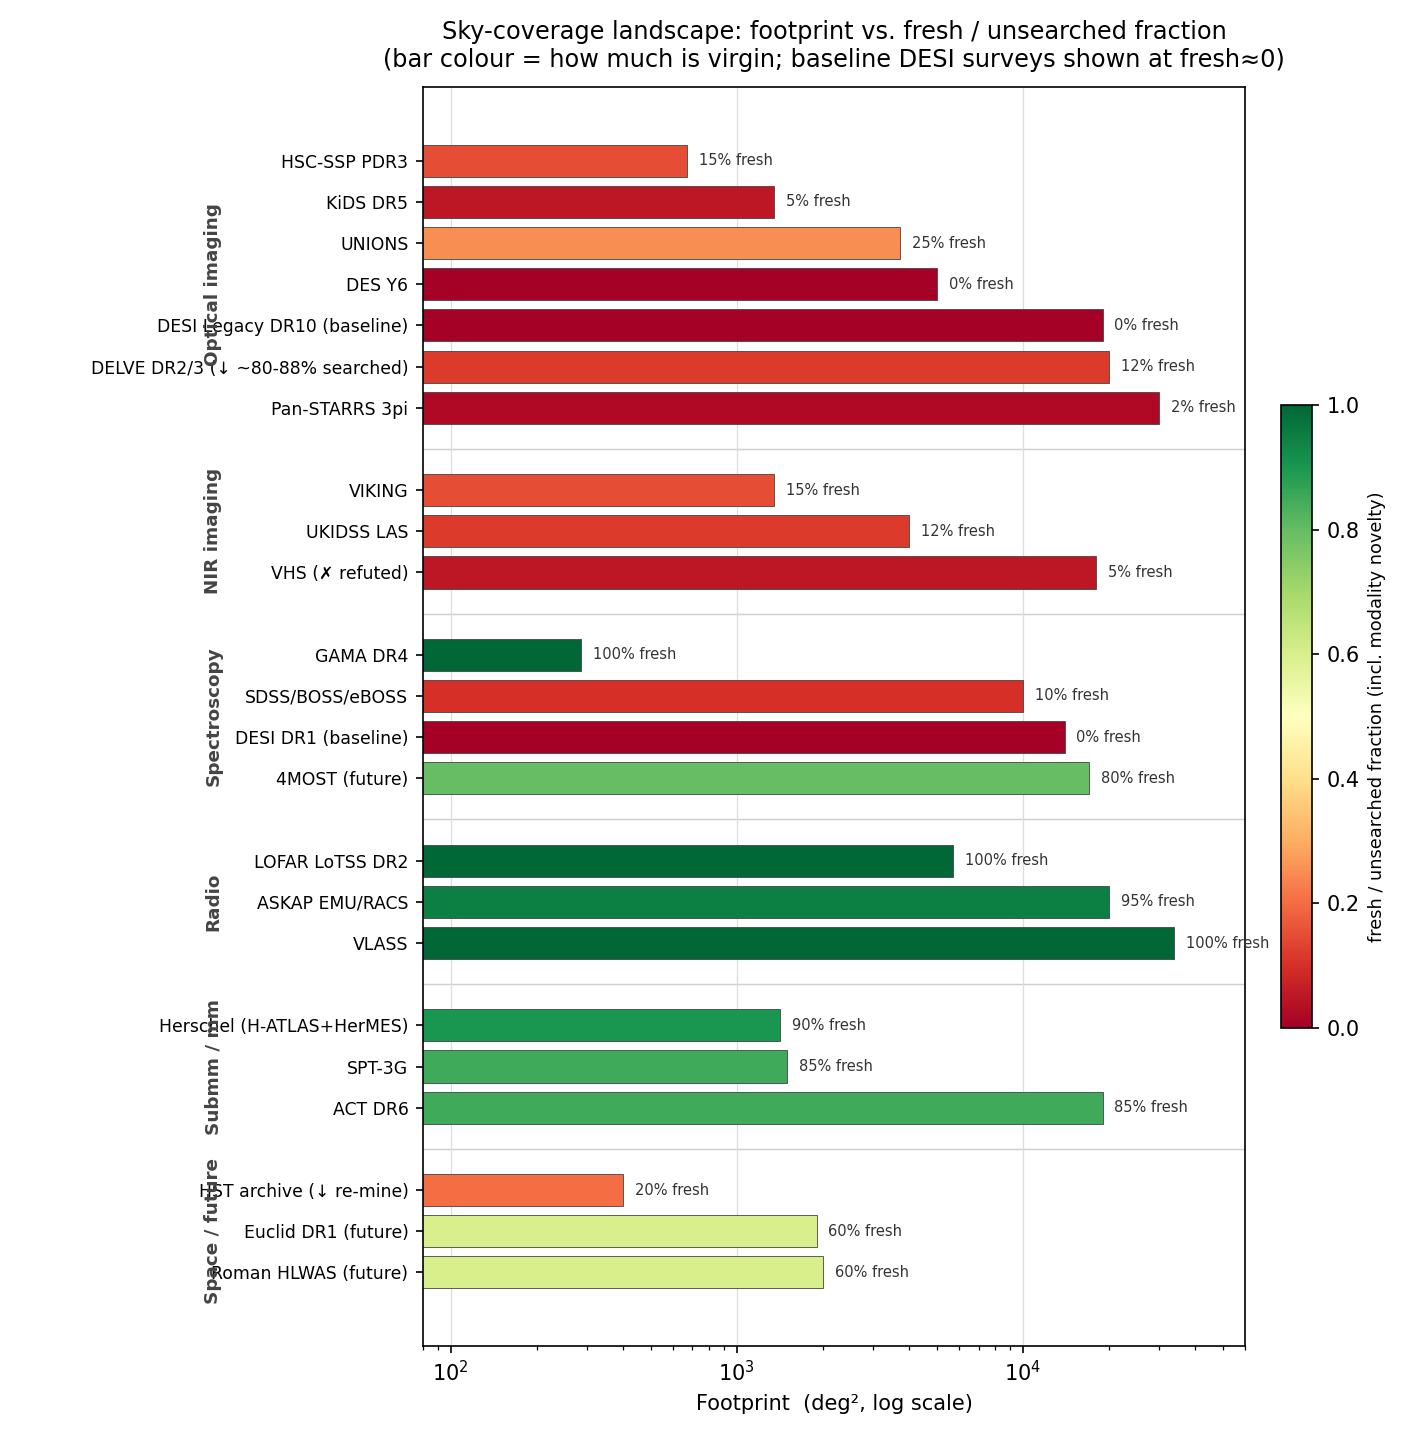
\includegraphics[width=0.96\linewidth]{figures/coverage_map.png}
\caption{Sky-coverage landscape: footprint (log deg$^2$) vs.\ fresh/unsearched fraction (bar
colour; includes modality novelty), grouped by modality. Baseline DESI surveys sit at
fresh$\approx$0 (red). The virgin reservoirs are wide-area radio (VLASS, EMU/RACS), the submm
modality, and the future
megasurveys.}
\label{fig:coverage}
\end{figure}

% ===========================================================================
\section{Findings by family}
% ===========================================================================
\subsection{Wide optical ground imaging --- mostly RED}
The southern DECam optical sky (DES, DESI-Legacy DR10-south, DELVE DR1) is the most
multiply-searched region in this study. DES Y6 is exhausted
\citep{jacobs2019a,jacobs2019b,rojas2022,odonnell2025}; HSC PDR3 is combed end-to-end
\citep{sonnenfeld2018,canameras2024sugohix,schuldt2025}; KiDS DR5 is done
\citep{petrillo2019,li2020,grespan2024}; UNIONS deep $gri$ was run by GLUE~I
\citep{savary2022,glue2025}. \survey{DELVE DR2} (first-scan score 61) was \textbf{downgraded} on
deep-dive (\S\ref{sec:pressuretest}): it tops out at $\delta\sim+30$ and Legacy DR10
\citep{inchausti2025} already searched $\sim$14{,}000\,deg$^2$ south of $+32$ \emph{using the same
ingested DELVE exposures}, so $\sim$80--88\% is already-searched sky; the genuine levers are the
\survey{DELVE DR3} deeper coadd and the low-$|b|$ frontier (a niche, not a fresh harvest;
\texttt{GAMA\_DELVE\_DEEPDIVE.md}). SkyMapper DR4 was \textbf{refuted} (seeing/depth make
galaxy-scale lensing unviable).

\subsection{Wide-area NIR ground imaging --- a modality gap with a \emph{physical} cause}
Nobody has run a blind wide-NIR lens search, and the VHS deep-dive shows \emph{why}: NIR is too
shallow to see the arcs. \survey{VHS} (\rgR\ \textbf{REFUTED} on deep-dive, 8 sources; first-scan
score 63 --- I initially rated it the top ``fresh far-south'' drop-in). \emph{(i) Depth kill-shot:}
$J_{\rm AB}\sim20.8$/$K_{s,\rm AB}\sim20.0$ (deepest $J\sim21.4$) is $\sim$3--4\,mag too shallow,
with no blue bands, so faint blue arcs fall below the limit --- a VHS CNN sees the deflector, not
the lens (no blind wide-NIR galaxy--galaxy catalogue has \emph{ever} been published). \emph{(ii) Not
fresh:} DECam reaches $\delta=-90\degree$; DELVE~DR2 ($\sim$21{,}000\,deg$^2$ griz) $+$ DES $+$
Legacy~DR10 blanket the southern sky 3--4\,mag deeper and mostly lens-searched, so net usable fresh
sky is $\sim$0--10\% (the unusable plane). Realistic yield $\sim$0--low-tens; the southern residual
it points to is re-running the optical CNN on \survey{DELVE DR2} griz, not a NIR search. \survey{VIKING}
is deeper ZYJHKs but its footprint \emph{is} the already-searched KiDS sky; \survey{VIKING/UKIDSS/
VIDEO} inherit the same NIR depth limit (\texttt{VHS\_DEEPDIVE.md}).

\subsection{Space high-resolution imaging --- mixed}
The contiguous deep fields are now swept (\citealt{nersesian2025cowls,nagam2025}; AnomalyMatch
2026). The \survey{HST general archive} looked like the best space drop-in, but the dedicated
pressure-test (\S\ref{sec:pressuretest}) \textbf{downgraded} it: HST is pencil-beam and not virgin
(Hubble Asteroid Hunter~II \citep{garvin2022} already scanned $\sim$27\,deg$^2$; COSMOS was already
CNN-searched \citep{pourrahmani2018,faure2008} and JWST-mined), so the realistic net-new yield is
tens--$\sim$150 secure via a completeness re-mine, not hundreds. \survey{JWST COSMOS-Web} is
re-searchable deeper than COWLS. The astrometric Gaia lensed-QSO search is mature
\citep{lemon2019,kronemartins2025gral9}. Euclid Q1 is exhausted \citep{euclidQ1A,euclidF}; Euclid
DR1 and Roman are future-watch.

\subsection{Optical spectroscopy --- FoF is the wrong tool; the blended channel is, and it is mined}
\survey{GAMA DR4} (first-scan score 64) was \textbf{refuted} on deep-dive
(\S\ref{sec:pressuretest}). Its multi-pass tiling does beat the fibre-collision wall, but
galaxy--galaxy lenses have $\theta_E\sim0.5$--$2\arcsec$, so the source lands inside one fibre ---
the two-fibre FoF channel cannot reach them. The channel that works is the single-fibre blended
spectrum, and \citet{holwerda2015} already executed it on GAMA; the same channel on DESI just
yielded 4{,}110 candidates \citep{desisinglefiber2025}. So GAMA's residual is wide/group-pairs $+$ a
confirmation/testbed role, and the scalable spectroscopic lever is a foundation-model
blended-spectrum re-mine, not FoF pairs.
\survey{SDSS/BOSS/eBOSS} ($\sim$5\,M public spectra, trivial access) is otherwise blocked: the
pairwise method is fibre-collision-limited and the single-fibre residual channel is exhausted
\citep{bolton2006,brownstein2012,shu2017,talbot2021,desisinglefiber2025} --- the only open lever
is a foundation-model re-mine (the natural SpectrumFM science target). \survey{LAMOST} adds
$\sim$30\% fresh objects over SDSS NGC at low resolution.

\subsection{Radio continuum --- the headline new-tooling opportunity (GREEN)}
No blind catalogue-scale radio strong-lens search has ever been published; the literature is
forecasts \citep{mckean2008,mccarty2024,rezaei2022}, known-lens cross-matches
\citep{martinez2024vlass}, or legacy lobe surveys \citep{browne2003class,phillips2001}.
\survey{VLASS} (33{,}885\,deg$^2$, public) offers a radio-source ML cross-match for blind
discovery \emph{and} a way to radio-confirm the program's existing optical candidates. The
\survey{LOFAR LoTSS} sub-arcsec ILT (uv-plane) path is the unbuilt high-yield lever
[O(10$^2$--10$^3$)]; \survey{ASKAP EMU/RACS} adds fresh southern radio sky.

\subsection{Submm / mm --- virgin modality plus a faint residual}
Bright-source submm lensing is famously complete (RED:
\citealt{negrello2010,negrello2017,nayyeri2016,wardlow2013,vieira2013,everett2020,reuter2020,canameras2015}),
but the \survey{ALMA Science Archive}$+$\survey{ALMACAL} \citep{oteo2016almacal} hold a petabyte
of interferometry \emph{never} systematically lens-searched (GREEN; uv-plane lens-finding).
\survey{SPT-3G} already has 4{,}303 extracted candidates \citep{archipley2024}; \survey{ACT DR6}
\citep{gralla2020} and \survey{Planck} \citep{trombetti2021} have similar faint residuals.

\subsection{Time-domain --- DOWNGRADED, but the strongest survivor (reframe to a Rubin precursor)}
\survey{ATLAS}/\survey{ZTF} were \textbf{downgraded} on deep-dive (\S\ref{sec:pressuretest};
\texttt{ATLAS\_ZTF\_DEEPDIVE.md}, 16 sources). ZTF's glSN content is \emph{saturated} (Magee 2023
full-archive $\to$0; AMPEL live; the group's own Park/Huang 2026 finder; 4 brokers
\citep{goobar2023,townsend2025}), and ``diff-imaging drops straight in'' is \emph{refuted} ---
ZTF/ATLAS already emit difference-image alerts $+$ forced photometry. Lensed-QSO discovery is
blocked by the $<2\arcsec$ resolution wall. \survey{ATLAS} is the one genuine under-searched glSN
channel but is depth-capped to a handful of extreme events. The defensible, forward-looking play is a
known-lens \textbf{watchlist} on the live broker/forced-phot streams $+$ a \textbf{SpectrumFM
spectral gate} --- a dress-rehearsal for \survey{Rubin/LSST} (the eventual prize, $\sim$100$\times$
rate, world-public alert stream, $\sim$1--2\,yr away).

\paragraph{Red-team outcomes.} Of 41 challenged opportunities: 34 CONFIRMED, 6 DOWNGRADED
(JWST-deep-fields$\to$red, SPT-3G$\to$yellow, Gaia-GraL$\to$yellow, ATLAS$\to$yellow,
HSC-PDR4$\to$yellow, VHS$\to$yellow), 1 REFUTED (SkyMapper$\to$red). The three surviving GREENs
(VLASS, ALMA archive, ALMACAL) each carry $\ge 5$ corroborating sources.

% ===========================================================================
\section{Cross-cutting analysis}
% ===========================================================================
\paragraph{Footprint overlap.} The most multiply-searched region is the southern DECam optical
sky (DES $\cup$ DESI-Legacy-DR10-south, which ingested DELVE/DeROSITAS exposures, $\cup$ DELVE
DR1). VST-ATLAS, SkyMapper and the southern PS1 strip all sit \emph{inside} this footprint
($\sim$0\% new sky). COSMOS ($\sim$2\,deg$^2$) is the single most-searched patch. The genuinely
virgin reservoirs are: fresh southern
radio (EMU/RACS, ACT-DR6); deeper mm (SPT-3G); the submm interferometric modality (ALMA/ALMACAL,
positionally decoupled from optical); all-sky time-domain \emph{content}; and the future
megasurveys. Key dedup facts: VIKING $\approx$ KiDS sky; UKIDSS LAS $\subset$ SDSS/DECaLS-north;
DELVE DR2/3 $\approx$ DES $\cup$ Legacy-DR10 (only $\sim$10--20\% net-new).

\paragraph{Method $\times$ modality.} Drop-in now (post-pressure-test): optical-cnn $\to$ DELVE DR3
(depth) $+$ low-$|b|$, J-PLUS/S-PLUS, JWST COSMOS-Web; spectro-fof $\to$ LAMOST $+$ GAMA wide-pairs
only; diff-imaging $\to$ ATLAS, ZTF, DECam-multi-epoch. \emph{Four first-scan candidates failed
scrutiny (\S\ref{sec:pressuretest}): HST archive (downgraded), VHS/wide-NIR (refuted --- too shallow
for arcs), GAMA DR4 (refuted for G-G --- FoF can't reach $\theta_E$; blended already done), and
DELVE DR2 as a fresh harvest (downgraded --- already in Legacy DR10).} Needs a build: SDSS/BOSS
(foundation-model blended-spectrum re-mine); all radio (source-match or uv-plane); all submm
(faint-DSFG selector or uv-plane); Gaia (astrometric ML). The highest-value builds are the VLASS
cross-match, the
ALMA/ALMACAL uv-plane lens-finder, the SPT-3G/Herschel faint-DSFG selector, and the SpectrumFM
SDSS/BOSS re-mine.

\paragraph{Searched-but-unpublished (direct-inquiry targets).} (1) SPT-3G's 4{,}303 strong-SMG
candidates \citep{archipley2024} were never published as a lens catalogue; (2) the Euclid
Discovery Engine consortium will sweep DR1 Wide internally around the Oct-2026 release;
(3) the GLUE/UNIONS group is searching embargoed multi-band data; (4) SuGOHI/HOLISMOKES will run
finders on the HSC PDR4 increment; (5) ACT DR6 has no published lensed-DSFG search beyond the
brightest-30; (6) Planck PCCS2 faint candidates ($\sim$50\% unconfirmed); (7) Gaia GravLens FPR
small-separation candidates lack a public confirmed catalogue.

% ===========================================================================
\section{Gaps the completeness critic found}
% ===========================================================================
The critic flagged $\sim$16 genuinely-missed datasets in three \emph{new families} the original
8 missed --- recommended as the next scan's seed list (Table~\ref{tab:critic}).

\begin{table}[h]
\centering\footnotesize
\caption{Critic-flagged additions (next-scan seed list).}\label{tab:critic}
\begin{tabular}{@{}lll@{}}
\toprule
Added dataset & New family & Why it matters \\ \midrule
WISE/unWISE/CatWISE2020 \citep{marocco2021catwise} & mid-IR all-sky cross-match & universal lens-vetting/counterpart layer \\
eROSITA eRASS1 DR1 \citep{merloni2024erass1} & X-ray & 12{,}247-cluster catalogue $=$ group/cluster lenses \\
NOIRLab Source Catalog DR2 \citep{nidever2021nsc} & ground optical cross-match & unified all-sky DECam base layer $+$ PMs \\
JCMT S2CLS \citep{geach2017s2cls} & deep ground submm & high-res lensed-DSFG number-count selector \\
HST/JWST grism; Euclid NISP grism & space slitless spectroscopy & blind emission-line lens discovery$+$confirmation \\
GMRT TGSS / GLEAM / Apertif & low-freq / southern radio & steep-spectrum lens cross-match \\
CFHTLS / CFHTLenS / SL2S & deep ground optical $+$ ML training & the canonical RingFinder training set \\
VLT/MUSE ($+$KMOS) ESO archive & optical IFU spectroscopy & de-facto confirmation $+$ serendipitous discovery \\
Quaia / Gaia$\times$WISE \citep{storeyfisher2024quaia} & all-sky lensed-QSO cross-match & ready-made quasar parent samples \\
Spitzer SWIRE/SERVS; J-PAS; Stripe~82; Chandra/4XMM; SO/CMB-S4 & various & secondary additions (see \texttt{OPPORTUNITIES.md}) \\
\bottomrule
\end{tabular}
\end{table}

% ===========================================================================
\section{Ranked action shortlist}
% ===========================================================================
\paragraph{Tier A --- drop-in now (public data, existing method), \emph{post-pressure-test}.}
After \textbf{five} deep-dives this tier is \emph{much smaller than the first scan implied} and is
best treated as prototype-scale (\S\ref{sec:synth}). Ordered by what survived:
(1)~\survey{ATLAS/ZTF} \textbf{reframed as a Rubin precursor} (the strongest survivor, but
\emph{downgraded}): do not re-run diff-imaging --- build a known-lens \textbf{watchlist} on the live
broker/forced-phot streams $+$ a \textbf{SpectrumFM spectral gate} $+$ an ATLAS extreme-mag glSN
sweep; best-justified because it is forward-looking (scales onto Rubin); (2)~\survey{DELVE DR3}
deeper pass $+$ low-$|b|$ frontier (\emph{downgraded} from DR2 ``fresh harvest''); (3)~\survey{JWST
COSMOS-Web} $\to$ deeper CNN (small field); (4)~\survey{J-PLUS/S-PLUS} narrow-band (speculative);
(5)~\survey{HST general archive} (\emph{downgraded}: completeness re-mine, best as the
HST$\to$Euclid/Roman readiness prototype); (6)~\survey{GAMA} (wide-pair $+$ confirmation layer $+$
blended testbed) and \survey{LAMOST}, DECam-multi-epoch --- supporting.
\emph{Refuted/downgraded out of the lead: VHS $+$ wide-NIR (too shallow for arcs), GAMA DR4 for
galaxy--galaxy (FoF can't reach $\theta_E$), DELVE DR2 as a fresh harvest (already in Legacy DR10),
and ZTF for blind glSN/lensed-QSO discovery (saturated $+$ resolution wall).}

\paragraph{Synthesis after five pressure-tests (the honest bottom line).}\label{sec:synth}
\emph{Every} current-data ``fresh public data $+$ existing method'' lead from the first scan was
downgraded or refuted (HST, VHS, GAMA, DELVE~DR2, ATLAS/ZTF --- 2 refuted, 3 downgraded).
\textbf{(1) Small current-data program (prototype-scale, now):} the \survey{ATLAS/ZTF}$\to$Rubin
precursor (watchlist $+$ SpectrumFM gate $+$ ATLAS extreme-mag glSN sweep --- the best-justified item
because it is forward-looking); \survey{DELVE DR3} depth $+$ low-$|b|$; \survey{GAMA}
confirmation/testbed; \survey{JWST COSMOS-Web}; \survey{J-PLUS/S-PLUS} --- realistic combined net-new
of order low hundreds, much of it transients.
\textbf{(2) The real, large opportunities} (unchanged --- never ``existing-technique'' claims): the
new-tooling green fields (\survey{VLASS}, the \survey{ALMA archive}/\survey{ALMACAL}, and the
\survey{SDSS/BOSS} SpectrumFM blended-spectrum re-mine) and pre-positioning for \survey{Euclid DR1}
/ \survey{Rubin} / \survey{Roman} / \survey{DESI DR2}, where the $10^3$--$10^5$ populations live.
\textbf{(3) Posture:} run the current-data items as readiness prototypes for the space-PSF CNN and
the alert-stream diff-imaging, while investing the real effort in the new-tooling builds and
megasurvey pre-positioning.

\paragraph{Tier B --- new-tooling now (public, real opportunity, build required).}
(1)~\survey{VLASS} radio cross-match ($+$ radio-confirm existing optical lenses);
(2)~\survey{ALMA archive}$+$\survey{ALMACAL} uv-plane lens-finder; (3)~\survey{SPT-3G}$+$%
\survey{Herschel} faint-DSFG selector (start by requesting the Archipley 4{,}303-candidate list);
(4)~\survey{SDSS/BOSS} foundation-model re-mine (the SpectrumFM science target);
(5)~\survey{EMU/RACS}, \survey{LoTSS-ILT}, \survey{ACT DR6}, \survey{Planck}.

\paragraph{Tier C --- pre-position for the future (inquiries $+$ readiness now).}
\survey{Euclid DR1 Wide} (2026-10-21; request early/joint consortium access);
\survey{Rubin/LSST} (connect to a broker; alert-stream diff-imaging is ready);
\survey{Roman HLWAS} (ready a space-PSF CNN; largest single ceiling);
\survey{DESI DR2} spectra ($\sim$2027; day-one FoF re-run);
\survey{4MOST} (the only large fresh \emph{southern} spectroscopy).

% ===========================================================================
\section{Future watch-list \& timeline}
% ===========================================================================
\begin{table}[h]
\centering\footnotesize
\caption{Future releases with expected public-availability and recommended action.}
\begin{tabular}{@{}llll@{}}
\toprule
Public & Dataset & Fit & Action \\ \midrule
2026\,Q3 (DP2) & Rubin/LSST (DR1 $\sim$2027) & Diff/CNN & broker connection; alert-stream diff-imaging \\
mid-2026 & 4MOST & FoF & southern FoF plan \\
2026 & WEAVE & FoF & monitor WAS public DRs \\
2026-10-21 & Euclid DR1 Wide & CNN/grism & early/joint consortium inquiry \\
unknown & HSC-SSP PDR4 & CNN & monitor; SuGOHI internal lists \\
$\sim$2027 & Subaru PFS (SSP) & FoF & SMOKA after 18-mo proprietary \\
launch by 2027 & Roman HLWAS$+$HLTDS & CNN/Diff & space-PSF CNN readiness \\
$\sim$2027 & DESI DR2 spectra & FoF & day-one Hsu-2025 FoF re-run \\
2026--2031 ops & DESI-II / Spec-S5 \citep{schlegel2025specs5} & FoF & long-horizon \\
online now & Simons Observatory LAT & New & monitor first mm catalogues \\
\bottomrule
\end{tabular}
\end{table}

% ===========================================================================
\appendix
\section{Data-access cookbook (selected public-now opportunities)}
% ===========================================================================
\noindent\textbf{Optical/NIR imaging.}
\survey{DELVE DR2/3}: NOIRLab Astro Data Lab SIA \url{https://datalab.noirlab.edu/sia/delve_dr3} $+$
TAP \url{https://datalab.noirlab.edu/tap} (anon; account for bulk).
\survey{VHS}: Astro Data Lab \url{https://datalab.noirlab.edu/vhsdr5.php} (TAP/SIA, anon).
\survey{VIKING}/\survey{UKIDSS}/\survey{VIDEO}: WFAU VSA/WSA \url{http://horus.roe.ac.uk/vsa/},
\url{http://wsa.roe.ac.uk/}.
\survey{J-PLUS/S-PLUS}: \url{https://splus.cloud/} ($+$ \texttt{splusdata} API).
\survey{HSC PDR3}: \url{https://hsc-release.mtk.nao.ac.jp/doc/} (free registration).
\survey{VST-ATLAS}: ESO Phase~3 $+$ WFAU OSA \url{http://osa.roe.ac.uk}.

\smallskip\noindent\textbf{Space imaging.}
\survey{HST HLA}: \url{https://hla.stsci.edu/} (anon).
\survey{JWST COSMOS-Web}: \url{https://exchg.calet.org/cosmosweb-public/DR1/}; deep fields via DJA
\url{https://dawn-cph.github.io/dja/}.
\survey{Euclid Q1/DR1}: ESA SAS \url{https://easidr.esac.esa.int/sas/} (free registration).
\survey{Gaia GraL}: Gaia Archive TAP \url{https://gea.esac.esa.int/archive/}.

\smallskip\noindent\textbf{Spectroscopy.}
\survey{SDSS/BOSS/eBOSS}: \url{https://www.sdss4.org/dr17/data_access/} (SAS bulk $+$ CAS TAP).
\survey{GAMA DR4}: \url{http://www.gama-survey.org/dr4/} (TAP $+$ bulk).
\survey{LAMOST}: \url{https://www.lamost.org/dr12/}.
\survey{DESI DR2}: \url{https://data.desi.lbl.gov/doc/releases/} (at release).

\smallskip\noindent\textbf{Radio.}
\survey{VLASS}: CIRADA/CADC cutout $+$ catalogs \url{https://cirada.ca/vlasscatalogueql0}.
\survey{LoTSS DR2}: \url{https://lofar-surveys.org/dr2_release.html}.
\survey{EMU/RACS}: CSIRO CASDA \url{https://research.csiro.au/casda/}.
\survey{MALS}: \url{https://mals.iucaa.in}.

\smallskip\noindent\textbf{Submm/mm.}
\survey{Herschel}: HeDaM \url{https://hedam.lam.fr/}.
\survey{SPT}: \url{https://pole.uchicago.edu/public/data/}.
\survey{ACT DR6}: \url{https://lambda.gsfc.nasa.gov/product/act/}.
\survey{Planck}: PLA \url{https://pla.esac.esa.int/}.
\survey{ALMA/ALMACAL/ALCS}: ASA \url{https://almascience.eso.org/asax/}, TAP
\url{https://almascience.eso.org/tap} ($+$ \texttt{ALminer}); calibrators have no proprietary period.

\smallskip\noindent\textbf{Time-domain.}
\survey{ATLAS}: forced-phot server \url{https://fallingstar-data.com/forcedphot/} (free reg).
\survey{ZTF}: IRSA \url{https://irsa.ipac.caltech.edu/Missions/ztf.html} $+$ brokers.
\survey{Gaia Alerts}: \url{http://gsaweb.ast.cam.ac.uk/alerts/}.
\survey{Rubin}: \url{https://dp1.lsst.io/} (alerts world-public via brokers).
\survey{DECam multi-epoch}: NOIRLab \url{https://astroarchive.noirlab.edu/}.

\smallskip\noindent\textbf{Critic-added archives (next scan).}
WISE/unWISE/CatWISE2020 (IRSA); eROSITA eRASS1 \url{https://erosita.mpe.mpg.de/dr1/};
NSC DR2 (Astro Data Lab); JCMT S2CLS (CADC JSA); HST/JWST grism (MAST); VLT/MUSE (ESO/AMUSED);
GMRT TGSS \url{https://tgssadr.strw.leidenuniv.nl/}; CFHTLS/SL2S (CADC); Quaia (Zenodo/VizieR).

\bigskip
\noindent\emph{The deep-research workflow gathered 147 unique prior-search references;
the subset that sets each survey's RED/YELLOW status is bibliographed below. See
\texttt{OPPORTUNITIES.md} for the complete annotated index with source URLs.}

\bibliographystyle{plainnat}
\bibliography{references}

\end{document}
